
\section{Applications: Active Debugging}
\label{sec:guided}

\iffalse
As discussed earlier, \parikshan will allow developers to have higher magnitude of instrumentation, making it easier to capture the causal flow and root causes of the problem.
However, this does not mean that an arbitrarily high amount of instrumentation can be used.
%In this section we explore automated techniques and guidelines to assist developers in using \parikshan for debugging their application.
%In this section, we explain adaptive instrumentation techniques which can help guide the debugger, while keeping the instrumentation within a pre-defined budget.
In this section we discuss how existing statistical debugging techniques can be applied to effectively isolate non-crashing bugs, using the budget limits described in the previous section.
\fi

\subsection{Overview}
\label{sec:guided_overview}


In the sections uptil now, we have introduced a framework for \livedebugging, a tool for instrumentation and mechanisms to configure the overhead budget of instrumentation. 
We now discuss some applications of \livedebugging in the real-world, and in particular introduce a new mechanism called \activedebugging.
The debug container allows for debuggers to apply any ad-hoc technique used in offline debugging. 
However, in order for us to have continuous debugging, it is essential to allow for forward progress in the debug container. 
Furthermore, the divergence due to instrumentation (either due to slowdown, or functional) should not stop forward-progress in the debug-container.

Having a debug-container which is isolated from the production, but still in sync with production services, allows a variety of ad-hoc debugging approaches to be integrated and leverage our framework.
Traditional offline debugging approaches, such as dynamic instrumentation can be easily directly applied to the debug-container without any ramifications. 
Others like memory or performance profiling, and execution traces can also be applied in the debug container.
Similarly the \debugcontainer can be used as a staging mechanism for record-replay on demand to ensure deterministic execution.
The key to applying these approaches is that none of them functionally modifies the application.

One possible route that we wish to explore further is how to allow for validation of test-cases, or validate functional patches/fixes, which may modify the output.
For the purposes of our exploration, we have currently assumed that these patches/and test-cases only bring about local changes, and not global changes in the application.
In this section, we introduce the concept of \activedebugging, whereby developers can apply a patch/fix or apply a test in the \debugcontainer.
\activedebugging ensures that any modifications in the \debugcontainer does not lead to a state change in the \productioncontainer.
This will enable the debugger to fix/patch or run test-cases in the debug-container while ensuring forward progress and in sync with production. 
We are inspired from existing perpetual invivo testing frameworks like INVITE~\cite{invivo}(which also provides partial test-isolation), in the production environment.

\iffalse
In recent years several monitoring techniques have been developed to monitor the health of production systems.
For example most modern operating systems have resource monitors~\cite{linuxHealth, windowsHealth, macHealth}, which can be used to track the CPU, memory usage, cache misses, temperature etc. of the physical machine.
These are useful to discover high workloads, or if the machine is stressed because of heavy resource usage.
Similarly, application level monitoring tools are used to report transactions or errors in the application.
Monitoring outputs usually provide the first clue towards resolving an error in the debugging process.
%While useful, these monitoring mechanisms  have a performance trade-off with the amount of instrumentation that can be done.
%Furthermore, the information provided by these logs may not be enough to understand the root-cause of the error.

However all monitoring/instrumentation techniques impose a performance overhead on the applications.
This can adversely impact user-experience, hence real-world production instrumentation is generally kept at very low levels.
\parikshan provides an alternative mechanism where this debugging/instrumentation can be done in parallel on a sandboxed cloned container.
Any instrumentation or monitoring in the debug-container has no performance impact on the production container.
In the context of our system, debuggers can use a variety of ad-hoc approaches to capture the root-cause of an error.
For example a naive approach could be to use trial-and-error instrumentation to find the execution trace for the error.
Alternatively, the user could also do aggressive brute force instrumentation for all function execution, which could help locate the problem.
However, both these approaches can have potentially high overheads, which in turn can lead to a buffer overflow.

In this chapter we introduce a statistical sampling approach which imposes a bounded performance overhead, to ensure maximal live debugging information, without causing a buffer overflow.
%In our search for more systematic approach towards live debugging, we looked towards two possible techniques.
%Firstly, we try to implement an automated budget limited instrumentation approach for capturing application logs.
We are inspired by previous work done in statistical debugging~\cite{cbi}, and delta debugging~\cite{delta} techniques which aim to streamline and automate the process of bug localization.
This is achieved by having predicate profiles from both successful and failing runs of a program and applying statistical techniques to pinpoint the cause of the failure.
The core advantage of statistical debugging is that the sampling frequency of the instrumentation can be decreased to reduce the instrumentation overhead.

One of the key criteria for successful statistical debugging is to have higher instrumentation rates, to make the results more statistically significant. 
There is a clear trade-off between instrumentation vs performance overhead for statistical instrumentation. 
A key advantage of using this with \parikshan is that we can provide live feedback based buffer size and bounded overheads, hence squeezing the maximum advantage out of statistical debugging without impacting the overhead. 
We evaluate the slack available in each request for instrumentation without risking a buffer overflow and getting out of sync of the production container.
Live interactive debugging provided by \parikshan further allows for quick updates to the instrumentation and targeting specific areas of the application code.
\fi
%\subsection{Background}
\label{sec:background-guided}

Before presenting our approach let us review basic concepts and terminology used in previous work in statistical/sampling based debugging approaches, and generating interesting predicates for capturing bugs.

\subsubsection{Terminology}
\label{sec: terminology-guided}


% ---- NIPUN -> THIS HAS BEEN COPIED IN PARTS FROM HOLMES BACKGROUND

The decision of what to monitor is crucial as the debugger can only decipher where the bug is located based on clues he  finds in the instrumentation output.
The decision of what to chose as an instrumentation point has been well studied in previous approaches \cite{}.
An \emph{instrumentation site} is a single program location at which the state of the running program will be inspected.
Instrumentation points are selected based on importance of the code location being tracked.
The idea behind instrumentation is to capture enough data to get a decent clue towards finding the bug.

Each of these instrumentation sites are decomposed into predicates which are conditionals with a true/false value.
Predicates can be branch conditionals, loops, function calls, return instructions and if conditionals.
Predicates provide significant advantages in terms of memory/performance overheads.
Instead of printing predicates, they are usually counted, and a profile is generated.
This reduces the amount of instrumentation overhead, and several predicates can easily be encoded in a small memory space.

Existing approaches also offer sampling as a means to more effective predicate instrumentation with minimal overhead.
This technique, creates instrumentation that yields a sparse but fair random subset of the complete counts.
Other approaches have extended this technique to adaptive automated sampling to better manage the overhead.

\subsubsection{Statistical Debugging}
\label{sec:Statistical Debugging}

% ---- NIPUN -> THIS HAS BEEN COPIED IN PARTS FROM HOLMES BACKGROUND

The Cooperative Bug Isolation Project forms the basis of our statistical debugging approach.
This project uses predicates at instrumentation points such as branch conditionals, call instructions etc., and statistically samples their counts to get a profile of the bug.
Each run of the program is further tagged with a feedback report for a single execution is a bit-vector with two bits for every path: one bit indicates whether the predicate was \emph{observed} and the other bit that indicates whether the predicate was executed in that run.
Predictors are scored based on \emph{sensitivity} (accounts for many failed runs) and \emph{specificity} (does not mis-predict failure in a successful run).
These scores are balanced using a numeric importance score computed as follows
The events corresponding to a predicate p from all the runs can be aggregated into four values: (1) $S_{o}(p)$: the number of successful runs in which the predicate p was observed (2) $F_{o}(p)$: the number of failed runs in which the predicate  p was observed (3) $S_{e}(p)$: the number of successful runs in which the predicate p was executed, and (4) $F_{e}(p)$: the number of failed runs in which the predicate p was executed.
Using these values, three scores of bug relevance are calculated.

\begin{equation}
    \label{eq:sensitivity}
    Sensitivity(p) = \frac{log|F_{e}(p)|}{log|F|}
\end{equation}

\begin{equation}
    \label{eq:context}
    Context(p) = \frac{F_{o}(p)}{S_{o}(p) + F_{o}(p)}
\end{equation}

\begin{equation}
    \label{eq:increase}
    Increase(p) = \frac{F_{e}(p)}{S_{e}(p) + F_{e}(p)} - Context(p)
\end{equation}

where F is the total number of failing runs. The harmonic mean of Sensitivity and Increase identifies predicates that are both highly sensitive and highly specific :

\begin{equation}
    \label{eq:importance}
    Importance = \frac{2}{\frac{1}{Sensitivity(p)}+\frac{1}{Increase(p)}}
\end{equation}

The Importance score is calculated for each path, and the top results are selected and presented to the programmer as potential root causes.

Nainar et Al\cite{}, further extend this approach in their work on adaptive statistical bug isolation.
They aim to reduce the instrumentation amount by initially instrumenting only a small part of the total predicates, then adaptively turn on the predicates which are more indicative of the error.
In particular, they define a vicinity function by which they aim to find predicates which are likely indicators of the error.
The main hypothesis is that predicates in the vicinity of existing predicates which are good error indicators, are also likely to be error indicators.

%\subsection{Statistical sampling of predicates with a bounded overhead}
\label{sec:guided_model}

In the previous chapter we discussed proposing a bounded overhead within which \parikshan can safely process logs, without requiring a re-cloning sync.
Here we use a statistical debugging approach which adheres to our bounded overhead.
We propose to assign to each predicate a weighted score which is associated with how frequently it should be monitored.
The sum of these weights will be equal to our bounded overhead.

In this work, we wish to establish a tradeoff between overhead of statistical debugging and the effectiveness of statistical debugging, at the same time maintaining a bounded overhead.
For instance, we can drop instrumentation of predicates which are executed more frequently to reduce the performance overhead in order to maintain our bounded overhead.
Program control and data flow inherently creates a hierarchical dependency between predicates, this can be leveraged in instrumentation to control the overhead, while at the same time provide some degree of clues to the debugger.

\subsubsection{Modeling the Target Application}

We define the program as a dynamic control-flow graph G \textless V,E \textgreater where V represent basic block entry points. 
The instrumentation granularity can be functional entries or conditionals which each should correspond to a basic block.
We call instrumentation points our predicates, where the predicate set \textless P \textgreater $\in$ \textless V \textgreater, 
i.e. each predicate can be an entry or exit point in the set of vertices's.


\subsubsection{Offline Profiling}

While not necessary, offline profiling of the target application can greatly assist in assigning weights to each predicate. 
Assuming that we have a representative input, the profile can be taken to show the time generally taken in each request, 
and every basic-block entry and exit point can be profiled to annotate time taken by each segment of the control path. 
While the processing time of each path can significantly differ depending on the input, 
we can get an approximate time taken by each section of the control flow graph for a large enough input set. 
This offline profiling helps us in assigning initial weights, and measuring the amount of slack available for each control-flow path.

\subsubsection{Assigning weight}

Weights can be defined to each predicate based on the following criteria:

\begin{itemize}
	
\item \textbf{Importance of the predicate itself}: 

The score for importance of a predicate can be defined similar to the Cooperative Bug Isolation Project (CBI) as shown in section ~\ref{sec:background-guided}. 

\begin{equation}
\label{eq:importance}
Importance = \frac{2}{\frac{1}{Sensitivity(p)}+\frac{1}{Increase(p)}}
\end{equation}


\item \textbf{Slack in context of the control flow path}: 

Model overall slack available based on offline instrumentation. 
 
\item \textbf{External factors}:

\end{itemize}

\textit{Amortizing Predicate Calculation}: Predicate scores are updated once every n runs

\subsubsection{Online Engine}

The job of the online engine is to decide whether or not a given predicate should be sampled. 
Inputs are 


\subsubsection{Cause Isolation}
\label{sec:cause_isolation}

Cause Isolation for bugs can be done in an adaptable manner. 

We assign weight W$_{i}$ to each predicate P$_{i}$ , where the weight denotes the sampling frequency.

\begin{equation}
    W_{i} = Probability\ that\ a\ predicate\ i\ is\ sampled
\end{equation}

\begin{equation}
    P_{i} = Instrumentation\ Overhead\ for\ Predicate\ i
\end{equation}

\begin{equation}
    \sum\limits_{i=1}^n W_{i}.P_{i} = Total\ Instrumentation\ Overhead\ Bound
\end{equation}

We have divided our approach in two halves, the first concentrates on statistical analysis for functional bugs.
Any application code can be modeled as a control flow graph 

\subsection{Motivating Example}
\label{sec:example}

We now discuss how live debugging can be used to find the cause of a bug using statistical debugging.
Take for example the code segment shown below:

\par
\begin{verbbox}[\footnotesize]
	void foo {
		if(x > num and f == NULL){
			x = 0;
			*f;
		}.
	}
\end{verbbox}
\fbox{\theverbbox}\par

In this code, the \texttt{*f} is clearly an erroneous call to this pointer, and will lead to an exception.
The function \texttt{foo}, can be called by various 

\subsection{Approach}
\label{sec:guided-approach}

In Figure~\ref{fig:offline-debugging}, we show the traditional mechanism of testing or validating patch/fixes in an application. 
In offline environments, developers apply patches and run the relevant inputs to verify that the patch works correctly. 
This is an interactive process, which allows one to verify the result and corrections before applying it to the production system.
Several cycles of this process is required, which may be followed by staged testing to ensure correctness before applying the update to the production.


\activedebugging (see figure~\ref{fig:active-debugging}) allows debuggers to apply fixes, modify binaries and apply hotpatches to applications. 
The main idea is to do a fork/exec, or parallel execution of an unmodified application.
The unmodified binary continues execution without any change in the input.
The debug-container should ideally mimic the behavior of the production, so as to allow for forward progress in the application as the debug-container will receive the same input as production.
The target process will be forked at the call of the testing function, the forked process can then be tested, the input can be transformed, or alternatively the same input can be used to validate any test-condition. 
At the end of the execution the test-process output can be checked and killed. 
The advantage of this technique is that any tests/fixes can be validated in the run-time environment itself.
This reduces the time to fix and resolve the error. 
The tests and fixes should have a local impact and should not be allowed to continue 

For Java programs, since there is no “fork”, we can utilize a JNI call to a simple native C program which executes the fork. 
Performing a fork creates a copy-on-write version of the original process, so that the process running the unit test has its own writable memory area and cannot affect the in-process memory of the original. 
Once the test is invoked, the application can continue its normal execution, while the unit test runs in the other process. 
Note that the application and the unit test run in parallel in two processes; the test does not block normal operation of the application after the fork is performed.

The fork-exec design of test-isolation ensures that the ``in-process'' memory of the process execution is effectively isolated. 
The production/debug containers are completely isolated hence the test does not impact the production in any way. 
To ensure further isolation, we propose to allow the test fork to only call wrapper libraries which allow write operations in a cloned cow filesystem.
This can be done using a COW supported filesystem with cloning functionality which are supported in ZFS and BTRFS.
For instance BTRFS provides a clone operation that atomically creates a copy-on-write snapshot of a file. By cloning the file system does not create a new link pointing to an existing inode; instead it creates a new inode that initially shares the same disk blocks with the original file. As a result cloning works only within the boundaries of the same BTRFS file system, and modifications to any of the cloned files are not visible to the original file and vice versa. 
This will ofcourse mean that we will constrain the debug/production environment to the File System of our choice.
We further propose that all test-cases in the debug-container share the test file system.

\begin{figure*}[h]
	\centering
	\begin{subfigure}[h]{0.25\textwidth}
		\centering
		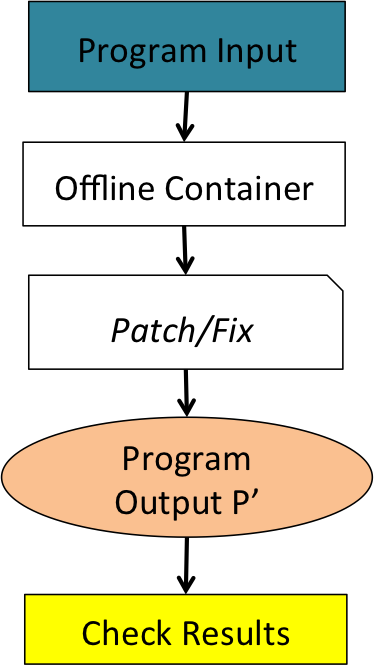
\includegraphics[width=0.95\textwidth]{guided/figs/offline.png}
		\caption{Offline Debugging}
		\label{fig:offline-debugging}
	\end{subfigure}%
	~ 	
	\begin{subfigure}[h]{0.75\textwidth}
		\centering
		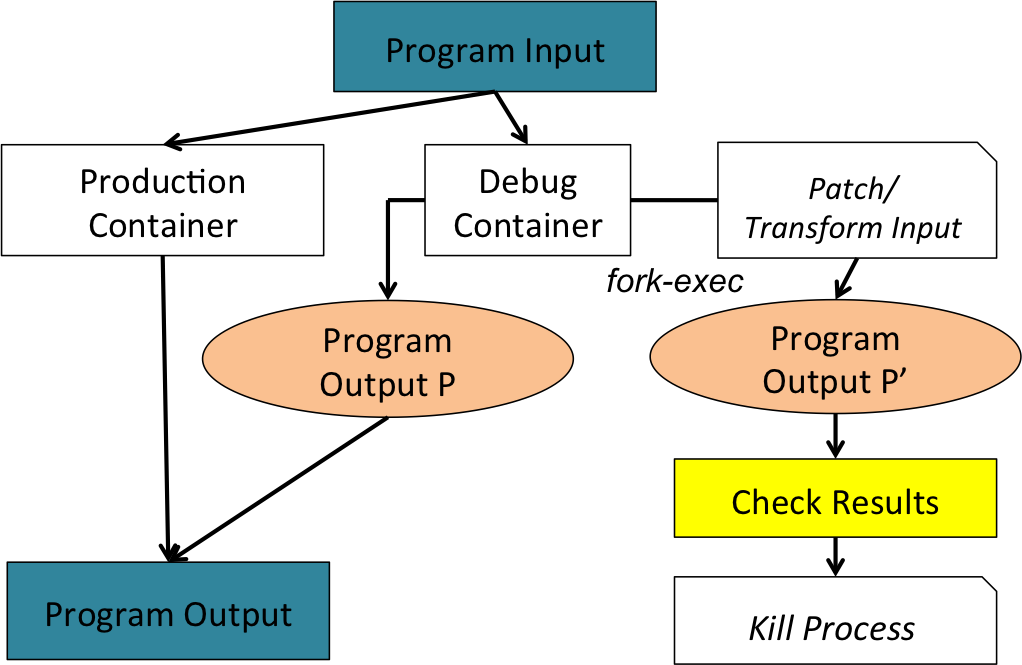
\includegraphics[width=0.95\textwidth]{guided/figs/active-debugging.png}
		\caption{Active Debugging}
		\label{fig:active-debugging}
	\end{subfigure}
	\caption{Debugging Strategies for Offline and Active Debugging}
\end{figure*}
\subsection{Feasibility}
\label{sec:guided_feasibility}

The current prototype for \activedebugging is in the early stages of development.
We have explored hotpatching in ~\cite{iprobe} and were able to successfully patch ELF binaries. 
Specifically our \iprobe tool enables dynamic instrumentation, and has been tested on several production level instrumentation techniques.
Other tools like Dyninst~\cite{dyninst}, and systemtap~\cite{systemtap} may also be used in tandem with ~\iprobe for our active debugging.

We have also explored previous approaches in the lab called INVITE (invivo testing~\cite{invivo}), which has looked into isolating test-cases in production environment. 
The core idea in invivo testing is to probabilistically trigger tests in the production environment. 
Furthermore, invivo ensures that these tests should not impact the production.
Other tools such as Java Assist, JAVA ASM also allow for binary modification and class re-loading in JAVA.
Applications like Tomcat, allow for dynamic class re-loading to speedup development. 
This inherently supports our design as we can design custom classes with forks which can do the test in the debug-container by generating two forks and killing them.
While complete isolation is not ensured in these approaches, forking execution does allow for process level isolation.
We have also explored file-system level isolation approaches using COW supported cloning mechanisms in BTRFS
The current approach will look at iteratively improving test-isolation guarantees in the debug-container, while the framework itself will provide complete isolation from production-container.
As part of the thesis we will integrate these approaches in the debug-container, and explore other applications for \livedebugging
